\chapter{Introduction and Background}
\label{chap:introduction}
Cultivation of grapes is one of the most economically significant crops in the world, as they are used for producing wine, juice, and also fresh fruit markets~\cite{mathew2025real}. However, as cultivation expands globally, disease issues increasingly threaten yield and quality, destabilizing the industry ~\cite{liu2025grape, mathew2025real}. Grape faces challenges from fungal and bacterial diseases including  Black Rot, Esca, Leaf Blight, and others can affect the entire harvest if not detected and managed promptly ~\cite{mathew2025real, talaat2025deepleaf, zhou2025lightweight, atesoglu2025detection}. The traditional disease identification relies on manual inspection by experts, which is laborious and vulnerable to error through human oversight~\cite{dharrao2025efficient}. In response to these limitations, The transition toward precision agriculture which is characterized by data driven management practices that has emerged as a critical paradigm shift to address these challenges~\cite{hnatiuc2023intelligent, aher2025deep}. Within this context, the development of intelligent monitoring systems capable of providing real time insights into plant health status has become increasingly vital for sustainable vineyard management.

The existing vineyard monitoring system is developed as a long-range, low-power wireless sensor network (WSN) platform for environmental monitoring and management of vineyards, aiming to provide methods to evaluate and improve the energy consumption of sensor nodes. The goal of this monitoring system is to provide an efficient and reliable way to promptly detect conditions adverse to grapes by measuring environmental data such as temperature, pressure, soil moisture, and humidity levels of vineyard fields. The platform is composed of a set of data acquisition sensors scattered over large open field areas, a gateway node, and a remote server to process and store the acquired data as shown in Figure~\ref{fig:lora}. This monitoring platform is based on the LoRaWAN specification, which is suitable for long-range and low-power lossy networks (LLNs) applications and provides a reliable link layer protocol for the deployed end nodes (sensor nodes) to access and transmit data to a central gateway, forming a star network topology~\cite{almufareh2024intelligent, jose2025lorawan}. The gateway node provides IP connectivity, forwarding the frames from the wireless sensor network to a local application server, which then sends the data to the LoRaWAN network server called The Things Stack. The telemetry data at the servers is gathered, stored in a MongoDB database, and displayed on a Grafana dashboard back to users, providing flexibility in the use and access of measured environmental conditions.

\begin{figure}[htbp]
   
    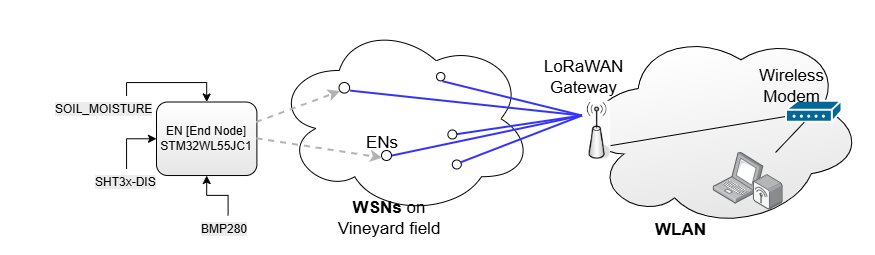
\includegraphics[width=0.7\linewidth]{images/lora2.drawio.png}
    \caption{\ LoRaWAN-based vineyard monitoring system architecture that only relies on environmental data for disease risk assessment}
    \label{fig:lora}
\end{figure}

Although the existing LoRaWAN-based vineyard monitoring system has showed significant potential for long term data collection across large field areas using low power communication, a fundamental limitation is still existing in this current implementations~\cite{gawande2024early, hnatiuc2023intelligent}. As some studies noted, a system with primarily rely on environmental data collection such as temperature, humidity, and pressure, transmitted over LoRaWAN networks and providing limited insights into the actual grapevine's health status~\cite{hnatiuc2025aiot}. Environmental sensing alone provides only indicators of disease risk rather than direct assessment of plant health. This gap of LoRaWAN-based vineyard monitoring system, not visualizing the actual grape leaf status, is representing there is a critical barrier to achieving more intelligent and responsive vineyard management systems.  


Meanwhile, deep learning models for identifying plant diseases have showed remarkable performance in laboratory and controlled environments. This is based on a comprehensive review of deep learning for grape leaf disease detection~\cite{aher2025deep}. This review shows convolutional neural networks and transformer based architectures can achieve high accuracy on detecting grape leaf diseases~\cite{karthik2024grapeleafnet, talaat2025deepleaf}. The Object detection frameworks such as YOLO also went further enabling automated leaf localization and disease symptoms in a complex field scenes~\cite{yang2024detection, chen2024yolov8}. Despite these advancements, the practice of deploying these models in vineyard monitoring systems remains limited due two critical challenges. First, The nature of  deep learning models typically demands high computational resources such as memory, processor and power, which is beyond the capabilities of the edge microcontroller~\cite{junaidi2025deep}. Second, the LoRaWAN network also have payload size constrains, transmitting raw image data is not feasible. 

Edge computing and lightweight deep learning (TinyML) becomes as a promising solution to address the computational resource and bandwidth limitations in LoRaWAN-based agricultural IoT systems. By performing image processing and inference at the sensor level. As prior studies explored, the lightweight vision models for disease detection in such resource-limited settings requires careful balance between model capacity and computational constraints~\cite{joshi2024edge, santhosh2024edge, junaidi2025deep}. However, most  of the  edge-based plant disease detection systems have been implemented on single-board computers such as Raspberry Pi or NVIDIA Jetson or smartphones, which offers mush more computational resources than microcontrollers~\cite{karim2024enhancing, lazcano2025deep, tao2025icrop+, mamun2025grape}.
 Therefore, such kinds of edge computing are not suitable for vineyard monitoring system which requires the edge computing for long term and battery powered deployment. 


To address this gap and to further enhance the intelligence of the existing vineyard monitoring system, this research came up with extension feature focused on edge computing for grape leaf disease detection. This extension Integrated edge AI at sensor level, moving beyond the traditional environmental monitoring, for nearly real-time visual-based insights into grapevines. By processing leaf images and running CNN classification model at the edge sensor, the system improves its ability to identify grape diseases. This differentiates the monitoring system from other systems that only rely on environmental data, thereby providing a more intelligent and efficient solution for vineyard management. This visual-based disease detection necessitates the tactical use of Edge AI computing to overcome the bandwidth limitations inherent in LoRaWAN communication for transmitting image data. Using ESP32-S3’s Edge AI capabilities, which support AI and can process images, the development process applied optimized configuration and enabled real-time grape leaf detection and classification directly at the edge sensor. This approach reduced power consumption by transmitting only the output of the MobileNet classification model, e.g. “Leaf Blight” with confidence 90\%, which is then seamlessly appended to the existing LoRaWAN data frame. Besides, by setting specified periodic intervals for image capture and on-device processing, followed by extended sleep periods (duty cycle operation) for the edge node, it aligns perfectly with a low-power, event-driven monitoring strategy, providing actionable insights while minimizing the impact on battery lifetime. Moreover, this comprehensive approach enhances the vineyard monitoring system by enabling early, localized detection of plant health issues, supporting more responsive and targeted interventions in precision agriculture.


Therefore, main aim of this research was to design, implement, and validate Edge AI system for grape leaf disease detection deployed on microcontroller within the existing LoRaWAN-based vineyard monitoring system. Specifically, this research introduces the direct visual-based disease detection into the existing environmental only monitoring system, by deploying a complete inference pipeline on ESP32-S3 microcontroller. Then the system integrates image acquisition, leaf localization within complex vineyard scenes, Multi-class disease classification, and inference results formatted to fit within LoRaWAN payload. Hence, contribution of this study have been diverse, addressing both technical and practical challenges of edge AI deployment for precision agriculture. It demonstrated feasibility of deploying these two-stage, object detection then classification pipeline on ESP32 microcontroller under strict  computing resources constraints.  This is a significant advancement beyond existing implementations that rely on powerful single-board computers or smartphone devices~\cite{karim2024enhancing, lazcano2025deep, mamun2025grape}.. Also introduces a weighted aggregation on the classification results from multiple leaves within a single frame, to send a compacted and robust results over LoRaWAN communication. overall, this work provide a complete system achitecture that fills the gap between enviromental only monitoring and direct disease detection. this research establised a foundation for Intelligent precision agricultural systems that combine the reliability of LoRaWAN with the optimized deep learning models deployed at the edge.

The Thesis organized in five chapters. Chapter 1 introduction and background of the research, outlining the research gap, main aim, and contributions of the study. Chapter 2 reviews some related works in the fields of IoT, LoRaWAN for precision agriculture, deep learning and edge computing for plants disease detection. Chapter 3 detailed system design implementation, including hardware selection, model architecture, dataset preparation, traning process, and integration with the existing LoRaWAN-based monitoring platform. Chapter 4 presents the experimental setup, evaluation metrics, and results of the system validation in both controlled and field conditions. Finally, Chapter 5 concludes the thesis by summarizing the findings, discussing implications for precision agriculture, and outlining directions for future research.

% The existing vineyard monitoring is developed in a long-range, low-power, wireless sensor network (WSN) platform for environmental monitoring and management of vineyards, aiming to provide methods to evaluate and improve the energy consumption of the sensor nodes. The goal of this monitoring system is to provide an efficient and reliable way to detect conditions adverse to the grapes by measuring environmental data such as temperature, pressure, soil mixture, and humidity levels of the vineyard fields. The platform is composed of a set of data acquisition sensors scattered over large open-field areas, a gateway node, and a remote server to process and store the acquired data. This monitoring platform is based on the LoRaWAN specification, which is suitable for long-range and low-power and lossy networks (LLNs) applications and provides a reliable link layer protocol for the deployed End Nodes (sensor nodes) to access and transmit data to a central gateway, forming a star network topology. The gateway node provides IP connectivity, forwarding the frames from the wireless sensor network (WSN) to a local application server, which then sends the data to the LoRaWAN Network server called The Things Stack Running from INFN's VM. The telemetry data at the servers is, gathered, stored in the MongoDB database, and displayed on the Grafana dashboard  back to the Users, providing flexibility in the use and access of the measured environmental conditions.

% Extension: Integrating Edge AI Computing for Grape Leaf Disease Detection
% To further enhance this vineyard monitoring system’s intelligence, this research adds an extension feature focused on edge computing for grape leaf disease detection. This feature Integrated edge AI at the sensor level, moving beyond the traditional environmental monitoring, for nearly real-time visual-based insights into grape leaves. By processing leaf images and running CNN classification model at the edge sensor, the system improves its ability to identify grape diseases. This differentiates the monitoring system from other systems that only rely on environmental data, thereby providing a more intelligent and efficient solution for vineyard management.

% The visual-based disease detection necessitates the tactical use of Edge AI computing to overcome the bandwidth limitations inherent in LoRaWAN communication for transmitting image data. Even though LoRaWAN excels at transmitting concise data frames for environmental readings, raw image transmission is too power-hungry and impractical for a low-power WSN. Utilizing the ESP32-S3’s Edge AI capabilities, which support AI and can process images, the development process becomes more flexible and efficient, enabling real-time grape leaf detection and classification directly at the edge sensor. This approach reduces power consumption by transmitting only the output of the clas- sification CNN, e.g. “Leaf Blight” with confidence 90\%, which is then seamlessly appended to the existing LoRaWAN data frame. Besides, by setting specified periodic intervals for image capture and on-device processing, followed by extended sleep periods (duty cycle operation) for the edge node, it aligns perfectly with a low-power, event-driven monitoring strategy, providing actionable insights while minimizing the impact on battery lifetime. Moreover, this comprehensive approach enhances the vineyard monitoring system by enabling early, localized detection of plant health issues, supporting more responsive and targeted interventions in precision agriculture.












